\documentclass[12pt]{report}
\usepackage{xcolor} % for different colour comments
\usepackage{parskip} % Space between each paragraph.
%\usepackage{hardwrap} % for text length of 80 pts
\usepackage[margin=1.2in]{geometry}
\usepackage{hyperref}
\usepackage{../ltx/edcomms}
\usepackage{graphicx}
\usepackage[section]{placeins} % Prevents floats from floating across sections
\usepackage{natbib}%Bibtex
\usepackage{float}
\usepackage{tabularx}
\usepackage{ltablex} %% Multi page tables 
\usepackage{booktabs}
\usepackage{amsfonts}
\usepackage{amssymb}
\usepackage{tabto}
\usepackage{tocloft} %% This package prevents table of contents from generating a page break
\usepackage{caption}
\usepackage{ifthen}
\usepackage{../ltx/edcomms}

%% Comments are enabled and disabled by 'draft' mode. I hacked in my own draft
%% mode (https://en.wikibooks.org/wiki/LaTeX/Macros) because the LaTeX draft
%% mode disables a bunch of things that I don't want it to. I just want it to
%% disable comments. Do not set any of this manually, just use the build script,
%% which builds both draft and final copies. Comments are enabled by default, so
%% if you build manually, you get a draft copy. 
\providecommand\draftmode{true}

\ifthenelse{\equal{\draftmode}{true}}{
\newcommand{\authornote}[3]{\textcolor{#1}{[#3 ---#2]}}
\newcommand{\todo}[1]{\textcolor{red}{[TODO: #1]}}
%\edcommstrue %% Dr. Kahl's comment package. Eventually we should migrate all
             %% comments to this.
}{
\edcommsfalse 
\newcommand{\authornote}[3]{}
\newcommand{\todo}[1]{}
}

% wss = Dr. Smith ; ds = Dr. Szymczak
\newcommand{\wss}[1]{\authornote{magenta}{SS}{#1}}
\newcommand{\ds}[1]{\authornote{blue}{DS}{#1}}


\usepackage{geometry}
\usepackage{changepage}
\setlength{\parindent}{15pt} % parskip sets this to 0. 15 is default.

\newcolumntype{C}[1]{>{\centering}p{#1}} %% For use with tabularx
%%%%%%%%%%%%%%%	START OF DOCUMENT %%%%%%%%%%%%%%%%%%%%
%% \edcommsfalse
\begin{document}

\pagenumbering{roman} %% Roman numerals before actual document starts
\begin{titlepage}\begin{center}
\thispagestyle{empty} %% No page no. on title

\vspace*{1cm}

{\Huge\textbf{Ampersand Event-Condition-Action Rules}}

\vspace{0.5cm}
{\Large Software Requirement Specification 
	
	\edinsert{JG}{Version 0 Revised}

\vspace{1.5cm}
Yuriy Toporovskyy,\ Yash Sapra,\ Jaeden Guo}
\vfill

We acknowledge that this document uses material from the Volere Requirements
Specification Template, copyright 1995 - 2012 the Atlantic Systems Guild
Limited.

\vspace{0.8cm}
\end{center}
CS 4ZP6 \\
October 9th, 2015 \\ 
Fall 2015 / Winter 2016 
\end{titlepage}

%% Revision history

\begin{table}[ht!]\begin{center}
\caption{Revision History}  
\begin{tabular}{|l|l|l|}\hline
\textbf{Author} & \textbf{Date} & \textbf{Comment} \\\hline 
Yuriy Toporovskyy & 26 / 09 / 2015 & Initial skeleton version \\\hline
Yuriy Toporovskyy & 30 / 09 / 2015 & Project drivers, description and \\ & & 
added project diagram and project flow chart \\\hline
J Guo & 09 / 10 / 2015 & Update: Non-Functional first half 4.1-4.3, added to 
1.2.2, \\ & & completed 2.2 \\\hline
J Guo & 13 / 10 / 2015 & Update: Figures added for Non-Functional 4.1-4.7,  \\ 
& & 
Non-Functional second half 4.4-4.7 half, \\ & & added Functional 3.3 - System 
requirements  and \\ 
& & diagram figure, \& Section 5.8 \\\hline
Yash Sapra &  12/ 09 / 2015 & Non-Functional - legal requirements, \\ & & Functional - User 
Requirements, tasks, risks \\ & & and chapter 5.
\\\hline
Yuriy Toporovskyy & 13 / 10 / 2015 & Initial round of editing \\\hline
J Guo & 04/ 02/ 2016 & Revision 0\\\hline
\end{tabular}
\end{center}\end{table}

\newpage

\tableofcontents
\listoffigures
\listoftables

\newpage
\pagenumbering{arabic} %% Arabic numerals in actual document

%%%%%%%%%%%%%%%%%%%%%%%%%%%%%%%%%%%%
%% Chapter 1: iNTRODUCTION        %%
%%%%%%%%%%%%%%%%%%%%%%%%%%%%%%%%%%%%
\setlength{\arrayrulewidth}{0.35mm}
\setlength{\tabcolsep}{16pt}
\renewcommand{\arraystretch}{2}
\begin{figure}
	\begin{adjustwidth}{-1cm}{}
	\begin{tabular}{ |m{4cm}|m{6cm}|m{4cm}|  }
		\hline
		\multicolumn{3}{|c|}{\bfseries{Project Time Table}} \\
		\hline
		\bfseries{Projected Finish Date}& \bfseries{Milestone} & 
		\bfseries{Actual Finish Date} \\
		\hline
		 09/10/2015& EFA SRS version 0 & 13/10/2015 \\
		19/10/2015 & EFA SRS version 1  & 22/10/2015 \\
		23/10/2015 & Proof of Concept Demonstation & 19/01/2016 \\
		11/02/2016 & Software Demonstration & 11/02/2016 \\
		%%--- & --- & --- \\
		01/04/2016 & EFA Complete & --- \\
		\hline
	\end{tabular}
	\end{adjustwidth}
\end{figure}
\chapter{Project Drivers}\label{ch:Intro}


\edcomm{YT}{Overall comments: 
  Do not use random words in places just to pad the line or whatever. 
  Use deliberate, consistent language. \\
  GRAMMAR PLEASE GOD GRAMMAR. Proofread your work! \\
  Do not make things up! I'm a little horrified 
  at how many things I found that were simply made up 
  and can be disproved in less than a minute of google 
  search \\ 
  ``Writing much, saying nothing'' - I see what our graders meant now.
  When you write a sentance you should be able to justify why each 
  and every single word is absolutely necessary. If it is not, 
  it should be removed. This goes back to being deliberate and 
  not just writing random crap. \\
  Formatting is extremely important! If your document looks good 
  but is really crap, you won't have a hard time tricking your reader
  into thinking it is actually good. Conversely, if your document
  looks like crap but is actually good, then noone will even 
  pay attention to the content and will focus on the crap formatting.
  In practice, the second thing DOES NOT HAPPEN. This is because
  very poor formatting is usually indicative of being in a rush 
  or a lack of effort,
  which also certainly wll reflect on the content of the document as well. 
  Also, do not assume that you can just ``do the formatting later'' or something. 
  Refactoring all the formatting of even a 1kloc tex document is non-trivial at best
  and a huge pain in the ass at worst. \\\\
  MOVING FORWARD:
  The biggest issue is the fact that the document has lost most semblance 
  of coherence and organization. There is no way to recover from this. 
  You can't really just keep throwing things in and hoping things will 
  make sense at the end. \\
  Take the template and create a skeleton (no content) for it. Include every single 
  section, without exception. Do NOT delete any sections from now on!
  Feel free to add whatever you like, or rename existing things,
  but do not reorganize or delete what is in the template. If you 
  do not know what to write for something, just skip it. 
  Once everything else is done, we can decide which sections 
  actually must be removed. 
  Now start copying thing from the current version of the document 
  to the skeleton, placing each thing in the appropriate section. 
  If you end up chaning the ordering of things, be careful 
  that you do not place an explanation which depends on another 
  before its dependency. Once you are done, you should have the 
  current document, but brought back closer to a state of organization. 
  }

\begin{figure}[!htb]
\centering
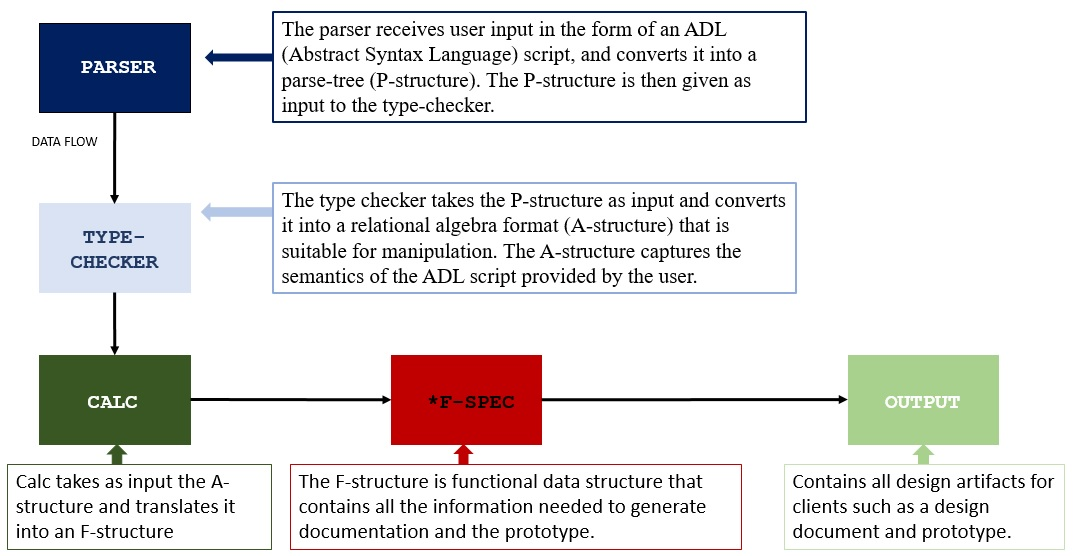
\includegraphics[width=\textwidth]{../figures/ampersand_parts}
\caption{Components of Ampersand System}~\label{fig:AmpersandParts}
\end{figure}

%%
%%\begin{figure}[!htb]
%%	\centering
%%	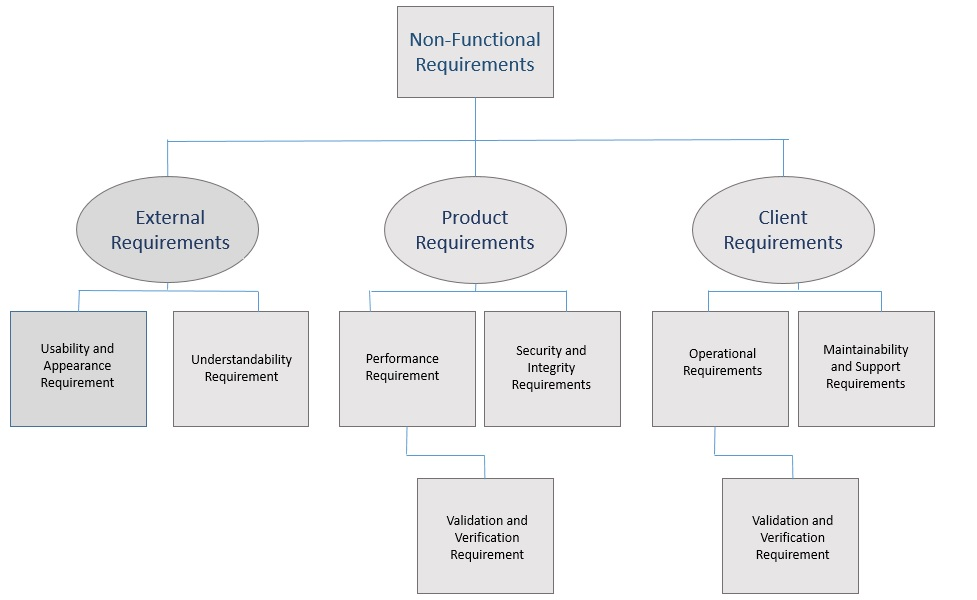
\includegraphics[width=0.8\textwidth]{../figures/NONFUNCTIONAL}
%%	\caption{Tree of non-functional requirements as it relates to EFA}~\label{fig:figure2}
%%\end{figure}
%%
\paragraph{}
\edcomm{YT}{What are specification details?} 
\edcomm{JG}{How everything works in Ampersand doesnt need to be included in an 
SRS concerning EFA, it'll bloat the document}

\edcomm{YT}{Essential how? This is far too little on the topic. I wrote quite
 a detailed explanation of how ECA fits into Ampersand for the original SRS,
 but it was deleted? Please fit it back in - as it stands nobody reading
 this document can have any idea as to what ECA does} 

\edcomm{JG}{You mean this intro? Its really long and complex, and dan said to 
simply it }

%% 1a. The User Business or Background of the Project Effort
A large part of designing software systems is requirements engineering. One
of the greatest challenges of requirements engineering is translating from
business requirements to a functional specification. Business requirements are
informal, with the intention of being easily understood by humans; however,
functional specifications are written in formal language to unambiguously 
capture attributes of the 
information system. Typically, this translation
of business requirements to a formal specification is done by a requirements
engineer, which can be prone to human error.

Ampersand is a tool which aims to address this problem in a different way; by
translating business requirements written in natural language into a formal
specification by means of a ``compilation process'' (\cite{derFun}). 
\edcomm{JG}{Maybe we should cut out how entirely, because there's a design 
    specification -- and solely focus on what? thoughts?}%
\edcomm{YT}{The significance of Ampersand has to do with how it solves the
    problem, or how it works. To speak to the purpose of the project means to
    explain why the Ampersand solution is good and why we are spending our time
    making it better. The rubric has a section titled 'General System
    Description', so we need to say something about it}%
%% NB: Put a tex comment at
%% the end of the line after your 'in-line' comments, or latex inserts extra
%% whitespace when rendering with comments off.
Even though the business requirements and formal specification are written in
entirely different languages, the ``compiler guarantees compliance between the
two'' (\cite[2]{derFun}). 

Ampersand also provides engineers with a variety of aids which
help them to design products that fulfill all of the needs of their clients and
the end-users (Figure~\ref{fig:figure1}); including data models, service 
catalogs and their
specifications. Requirements engineering is perhaps most important in
safety-critical systems; to this end, Ampersand generates modeling aids and
specifications which are provably correct (\cite{derFun}). 

\begin{figure}
    \centering
    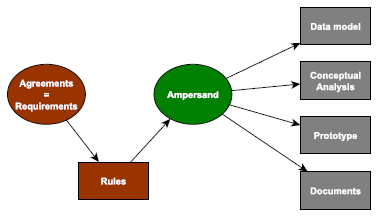
\includegraphics[width=0.7\textwidth]{../figures/ampersand_artifacts}
    \caption{Ampersand produces a set of artifacts based on user's 
    requirements.}~\label{fig:figure1}
\end{figure}

%% 1b. Goals of the Project 
Ampersand has proven reliable in practical situations, and there have been
efforts to teach this approach to business analysts. A large portion of the
Ampersand system is already in place; the primary focus of this project is to
augment Ampersand with increased capabilities for automation.

For example, consider a system for ordering products online. Ampersand takes, as
an input, statements of business requirements like
\edcomm{JG}{Good example, could we put something in here about restrictions of 
    of the real world?}%
\edcomm{YT}{Business requirements *are* real world requirements. Do you mean 
something safety-related?
    This example isn't the best, I know, but I deliberately chose a simple 
    example}%
\edcomm{YS}{The example is easy to understand. I think we should keep it.} 
\edcomm{YS}{I'm not too sure if the haskell implementation needs to be a part 
of the introduction.
    Rubrics indicate the following critera - - - - %%%%%%%%%%%%%%%%%
    delineate purpose, specify intended audience), system scope, definitions, 
    acronyms,
    abbreviations, references, system overview, roadmap of report - - - -
    %%%%%%%%%%%%%%%%%%%%%%%
    I believe we miss definition of EFA and ECA since it is being used a lot in 
    the document
}%
\edcomm{YT}{Haskell isn't mentioned at all the intro, ECA is mentioned but is 
also defined
    (it is really quite simple, we don't define it mathematically, just in 
    natural language, so 
    it shouldn't be incomprehensible).}%
\begin{quotation}
    \noindent{\emph{Every order must have a customer and a list of products; 
    and the total price on
            the order must equal the sum of the prices of the products.}}
\end{quotation}
\edcomm{YS}{Attempt at defining ECA}%
\edcomm{YS}{Should we remove some of the haskell code and define the scope of 
    our project in terms of conserving these data rules instead? There's a good 
    chance Dan hasn't read our new problem statement so he doesn't necessarily 
    have 
    a clear idea of Ampersand. Suggestions?}
\edcomm{YT}{There is no Haskell code!}
\edcomm{YS}{Sorry, i meant the pre-post conditions pairs, I guess we'll let 
    that stay.}%

The requirements engineer formalizes this requirement
as a rule in Ampersand, which is a constraint on the data in the database.
These constraints are called invariants, because they are meant to remain 
satisfied at
all times during runtime.

The Ampersand compiler translates each rule into Event-Condition-Action Rules 
(referred to as ECA rules hereafter).
An ECA-rule specifies the action to be taken by the system when an event takes 
place
under a given condition. In Ampersand, the purpose of an ECA-rule is to restore
invariants, i.e. to change data in the database such that the constraint 
becomes true
again, after having been violated. Currently, an information system generated by
Ampersand produces runtime events that signal violations of the constraints. 

It also contains the ECA rules that are generated by the Ampersand compiler --
information about ECA rules is propagated
\ds{``propagated"}
through the pipeline. 
\ds{``pipeline"?} 
of
Ampersand. However, these ECA rules are not being called in order to restore
violations automatically in the current version of Ampersand. This is due to the
fact that it is currently unclear how to incorporate the functionality of ECA
rules into the information system generated by Ampersand. 

The information system may contain a function for manipulating orders. 
(Ampersand can also generate
prototype software models, including functions types like these, from business
requirements - but this is not the topic of our contribution). For example,

\begin{verbatim}
addToOrder : ( o : Ref Order, t : Product )
\end{verbatim}
\noindent{where \verb|Ref x| represents the type of references to values of type
    \verb|x|; \verb|Order| and \verb|Product| the types of orders and products, 
    respectively.  }

Ampersand can generate pre- and post-conditions for this function, based on the
business requirements. This constitutes a formal specification of the
information system. For example, the above function may have the following 
specification:

\begin{verbatim}
{ PRE: o.totalCost = t0 } 
addToOrder(o,t) = ...
{ POST: o.totalCost = t0 + t.cost } 
\end{verbatim}

It is proven \edcomm{YT}{This is 'proven' because someone told me we have a
    proof/presentation of the algorithm, but not its implementation. Can anyone
    find this? We absolutely need a reference to this.} 
\edcomm{JG}{Can you give me more context as to what is proven? I found an 
    article on ampersand subsets, I pushed it; look for "subsets" by 
    Joosten(both)}%
\edcomm{YT}{There is no file in the repository with the word 'subset' in it?}%
\edcomm{JG}{Sorry, look for domain, it may help}
that for the subset of processes which Ampersand can support, there is an
algorithm which will generate the necessary code to satisfy the post-conditions
(i.e. 
\ds{``i.e."}
formal specifications) of each function. However, Ampersand does not yet
implement this algorithm. Currently, a user of Ampersand must manually indicate
how each violation must be corrected.

In the previous example, the implementation of the
function could be as follows: 

\begin{verbatim}
{ PRE: o.totalCost = t0 } 
addToOrder(o,t) = 
o.orders.append(t);
o.totalCost = o.totalCost + t.cost;
{ POST: o.totalCost = t0 + t.cost } 
\end{verbatim}
\edcomm{JG}{Should pieces of code be left to design spec?}
The first line includes the item in the order, and the second line fixes the
violation of the post-condition which would occur without it. Currently this
second line would have to be hand-written by the programmer, but the
aforementioned
\ds{``aforementioned"}
\edcomm{YT}{Should have a name to refer to the algorithm
    somehow?} algorithm can derive it from the business rules. The main
contribution of this project will be to implement the algorithm which generates
the code to fix violations.

\ds{You may want to simplify the introduction a bit to make the purpose more 
clear.}
\edcomm{JG}{I tried addressing this -- its still not addressed. }
{\section{The Ampersand Environment}\label{sec:Purpose}}
Ampersand is a on-going project with an increasing number of modules being
added to it on a weekly basis. 
\edcomm{YT}{Is this really true? Will it always be true? I know you are 
 going for dramatic effect, but a technical document isn't really the place}
\edcomm{JG}{Wow, really? wasn't going for dramatic effect, its just saying 
we're working with a system thats not yet complete. every time i pull there's 
several additions in the main branch and this criticism isn't constructive 
towards.. anything.}
Since this project focuses on a component of 
Ampersand, it must be built to fit within the Ampersand environment and 
co-exist with other modules.
\edcomm{YT}{The last sentance is quite akward, it can probably just be removed
 or reworded to not include the examples which are obviously mentioned further on}
\subsection{Project Purpose}

\edcomm{YT}{Again, this says almost nothing. See previous comment about 
  detailed explanation of ECA}
\subsection{Project Goals} 
The goals of this project is to implement a design for an internal component 
that translates ECA rules to SQL queries that is both maintainable and provably 
correct.
\edcomm{YT}{We are designing part of a real software system
  for a real software tool. Anything ``capstone'' is unrelated 
  and should be removed}

\edcomm{YT}{Same thing about far too little information. Provable correctness?
  You do not design code, you write code based on a design. We are 
  not ``designing'' anything, unless you call implementation details 
  a ``design''. }

\section{The Stakeholders}\label{sec:Stakeholders}
The stakeholders are separated into two sections, those that directly benefit 
from this projects contribution and those that indirectly benefit.
\subsection{Ampersand Designers}\label{subsec:Ampersand}
Ampersand designers are our client, and they directly benefit from this project 
as it bring Ampersand one step closer to completion. 

\eddelete{YT}{This project EFA (ECA for 
Ampersand) delivers a maintainable component for Ampersand that produces type 
safe SQL queries, which will be used to maintain the consistency of the data in the back-end Database. 
}
\edcomm{YT}{A whole bunch of words which say nothing. Please reword}
\edcomm{JG}{suggestions? }

\subsection{End-Users}\label{subsec:BusReq}
\paragraph{}
Ampersand users indirectly benefit from this project's contribution because it 
drastically decreases the time spent manually restoring system invariants, 
which are the rules that maintain the validity of each business process. 
\edcomm{YT}{The time spent restoring invariants manually is always 0. It is the 
 time spent writing ugly PHP code in order to restore invariants.}
\edcomm{JG}{did you want me to add "writing PHP code to restore invariants"?}
As EFA is 
executed during compile time, the user will not suffer any noticeable delays 
and can rest assured that the artifacts they received are correct according to 
specification.
\edcomm{YT}{What???? How can we execute SQL on the database at compile time?
  This is just a complete lie!}
\edcomm{JG}{no it says that EFA is executed as in called during compile time, 
not that SQL queries are generated and sent during compile time.. Does it not 
have to compile for EFA to kick in? }

%%%%%%%%%%%%%%%%%%%%%%%%%%%%%%%%%%%%
%% Chapter 2: Project Constraints %%
%%%%%%%%%%%%%%%%%%%%%%%%%%%%%%%%%%%%
\chapter{Project Constraints}\label{ch:Constraints}
The current Ampersand system is the main limitation of this project; 
\edcomm{YT}{``limitation'' is not the right word here.}
\edcomm{JG}{Incase this wasnt clear, I dont *intentionally* put things in here 
knowing they are wrong, simply telling someone they're wrong doesnt help them 
get it right. When you teach a kid to tie their shoes, just telling them 
they're wrong -- doesnt help them do it right. So how about you tell me why its 
wrong, and suggest other things that make it right?}
everything 
that is built, must be built to fit within its current constraints. These 
constraints include the language used to build Ampersand (i.e. Haskell). 

\eddelete{YT}{Anything incorporated into Ampersand must be implemented in the Haskell 
language.}
\edcomm{YT}{This was JUST said. DNRY!!!!!!!!!!!}
\edcomm{JG}{what is dnry?}
An additional constraint placed on 
this project by our clients is to produce maintainable 
code; this includes the use of support modules such as external libraries
generated by this project to help translate ECA rules to SQL queries.
\edcomm{YT}{I'm not sure what this is trying to say.
  ``support modules'' - what about them? 
  You are saying ``this includes'' ... ``support modules'' - which 
  doesn't even make sense}

\section{Mandated Constraints}\label{sec:Constraints}
%%%%
%% 4.1 Solution constraints. 

All code must be well documented, backwards compatible and fit seamlessly into 
the current Ampersand project. Due to the long-term nature of this project, we 
must minimize the number of external dependencies. 

%%3b.
\subsection{Implementation Environment of the Current System}
\subsubsection*{Haskell}
The Ampersand code base is written almost entirely in Haskell 
(\cite{ampSource}) with the exception of user interfaces for the generated 
prototypes written in PHP and Javascript. Additional code is required for the 
prototype, however Haskell is the main programming 
language we use to build modules for Ampersand. 

\edcomm{YT}{Mention that we may have to write code for the prototype as well
 , but it probably won't be much.}
\edcomm{JG}{done.}

\subsubsection*{The Glasgow Haskell Compiler \& Cabal Build System}
The GHC and Cabal build work in unison to compile Ampersand source code. 

\edcomm{YT}{GRAMMAR! This sentance is BAD. A lot of the sentances lack the 
  basic essential component of grammatical correctness. I can't correct 
  each one so please proofread for grammar!}

The Glasgow Haskell Compiler 7.10 (\cite{GHC}) with the Cabal build 
system (see \verb|ampersand.cabal| must be used to compile Ampersand 
\cite{ampSource}). Ampersand is not designed to used with other Haskell 
compilers. \edcomm{YT}{Mention versions}


\subsubsection*{GitHub Repository}
All source code is hosted on GitHub for both the Ampersand main branch and this 
project's personal repository.
\edcomm{YT}{GRAMMAR}

\subsubsection*{Graphviz}
Graphviz is an open source graph visualization software, which can
visually represent information in the form of charts and graphs. Graphviz is 
used to create visuals in Ampersand artifacts and is essential to running 
Ampersand.

%%removed XAMPP, not a constraint

\subsection{Partner of Collaborative Applications}
\edcomm{YT}{``Partner of Collaborative Applications'' - what}

\edcomm{JG}{3c. of voltere template, applications that are not part of product 
but with which the product will collaborate, can be external applications, 
commercial packages or pre-existing in-house applications}


\edcomm{YT}{This entire table is no good. A table is not the 
 right format for a module heirarchy. See email}
\begin{longtable}{ |m{4.5cm}|m{1.5cm}|m{7cm}|  }
    \hline 
    \textbf{Name} & \textbf{Type} & \textbf{Description} \\ \hline \hline
    AbstractSyntaxTree & Ampersand module & A module designed specifically for 
    Ampersand, data from this module is manipulated in EFA.
    \\ \hline        
    Control.Applicative & Library module & An interface that provides an 
    intermediate structure between a monad and a functor. 
\edcomm{YT}{NONONONO never write the words ``monad'' or ``functor'' or ``applicative'' in this document 
  unless you are willing to write a section for the appendix explaining 
  category theory!}

This interface is 
    used to embed pure expressions, sequence computations and combine their 
    results.  \\ \hline
    Control.Exception & Library module & An interface that provides support for 
    raising and catching build-in and user-defined exceptions.  \\ \hline
    Control.DeepSeq & Library module & 
\edchange{YT}{This module is used to fully evaluate 
    data structure and is used to prevent resource leaks in lazy IO programs.  }
{ This module provides a type class for evaluating data to normal form.
}
    \\ \hline            
    Data.Proxy & Library module & A concrete proxy type, 
\edchange{YT}{used to represent the 
    value of something else.}  
{ used to explicitly manipulate type parameters. }
\edcomm{YT}{``represent the value of something else'' is literally
  one of the vaguest things I've ever heard}
\edcomm{JG}{Thats from hackage, sounds like a proxy}
\\ \hline    
    Data.Type.Equality & Library module & 
\edchange{YT}{This module offers pattern-matching 
    on types and provides a proof, 
it is used as a definition of propositional 
    equality.}{This modules defines a proposotional equality type} 
\edcomm{YT}{This doesn't make much sense. Please don't write things that 
  don't make sense just to write something} 
\edcomm{JG}{this is all from hackage} \\ \hline        
    Data.List & Library module & A module that provides support for operations 
    on list structures.  \\ \hline
    Data.Char & Library module & A module that provides support for characters 
    and operations on characters.  \\ \hline
    Data.Coerce & Library module & Provides safe coercions between data types; 
    allows user to safely convert between values of type that have the same 
    representation with no run-time overhead.   \\ \hline
    Debug.Trace & Library module & Interface for tracing and monitoring 
    execution, used for investigating bugs and other performance issues.  \\ 
    \hline
    GHC.TypeLits & Library module & Internal GHC module that declares the 
    constants used in type-level implementation of natural numbers.  \\ 
    \hline    
    GHC.Exts & Library module & 
\edchange{YT}{This modules allows the use of pointers to an 
    object or array of objects. }  
{ This module provides access to types, classes, and functions necessary to 
  use GHC extensions. }
\edcomm{YT}{Again with the writing random stuff.... if you had googled
  ``GHC.Exts'' you could discover precisely what it 
  does in 10 second, so this is just plain lazy}
\edcomm{JG}{It gives you 
https://www.haskell.org/hugs/pages/libraries/base/GHC-Exts.html, which then you 
need to google GHC Extensions cause all it tells you is that its an approved 
way of getting extensions -- which doesnt tell you anything, and a Ptr A value 
of type Ptr a represents a pointer to an object, or an array of objects, which 
may be marshalled to or from Haskell values of type a.
    
    The type a will often be an instance of class Storable which provides the 
    marshalling operations. However this is not essential, and you can provide 
    your own operations to access the pointer. For example you might write 
    small foreign functions to get or set the fields of a C struct. is a data 
    type in Exts, so no I wasnt lazy, wrong but not lazy.  }
 \\ \hline    
    Language.SQL.SimpleSQL & Library module & Syntax: provides the AST for SQL 
    queries. \\& & Pretty: provides pretty printing functions that formates 
    output for human reading. \\ \hline            
    Numeric.Natural & Library module & Natural number type  \\ \hline    
    Prelude & Library module & A standard module that is imported by default 
    and provides support for basic data types, comparison functions, and 
    methods used for data manipulation.   \\ \hline
    System.IO.Unsafe & Library module & This module allows IO computation to be 
    performed at any time.\\ \hline
\eddelete{YT}{, the IO computation must be free of side effecets and 
    independent of its environment to be considered safe. Any I/O computation 
    that is wrapped in unsafePerformIO performs side effects.  }
\edcomm{YT}{This is not the place for this detail, and the 2nd part is simply untrue again}

    Text.PrettyPrint.Leijen & Library module & A pretty printer module based 
    off of Philip Wadler's 1997 "A prettier printer", used to show SQL queries 
    in a readable manner to humans \cite{hackage}. \\ \hline 
\edcomm{YT}{If you are going to cite ANYTHING do it properly! This is no good}
        
    Unsafe.Coerce & Library module & A helper module that converts a value from 
    any type to any other type. The user must assure that the old data type and 
    the new data type have identical runtime representations, else undefined
    behaviour occurs.\\  
\eddelete{YT}{This is used in the translation of ECA rules to SQL 
    using user-defined data types.}
\edcomm{YT}{This doesn't mean anything. What is a unique datatype?}
\edcomm{JG}{unique=user defined}
\end{longtable}
\section{Naming Conventions and Terminology}\label{sec:Naming} 

\edcomm{YT}{This section is in desperate need of being revised. 
  Please collect all the definitions you can find in this doc
  which should be here (anything even vaguely math or Haskell related
  should be here!). If you think the actual definition is too hard 
  to write, just leave it blank (I'll fill it in)}

\begin{description}
\item[ECA] Stands for Event-Condition Action. The rule structure used for data
  bases and commonly used in market ready business rule engines. ECA rules are
  used in Ampersand to describe how a database should be modified in response to
  a system constraint becoming untrue.
  
\item [ADL] Stands for ``Abstract Data Language'' (\cite[13]{derFun}). From a
given set of formally defined business requirements, Ampersand generates a
functional specification consisting of a data model, a service catalog, a
formal specification of the services, and a function point analysis. An ADL
script acts as an input for Ampersand. An ADL file consists of a plain ASCII
text file.
\item [Ampersand] Ampersand is a method and the name of the open source 
project. 
    \begin{itemize}
        \item[$\Rightarrow$] The Ampersand method is used to generate
        functional specification from formalized business requirements.
        \item[$\Rightarrow$] The Ampersand software is a tool that implements 
        this method.
    \end{itemize} 
    
\item [Business rules] Rules that exist to represent real world 
constraints that the virtual world does not naturally possess, such as resource 
and social limitations. Examples of constraints include but are not limited to 
financial, logistic, physical or legal constraints.

\item [EFA] Stands for ``ECA (see above) for Ampersand''. This term is used to 
refer to this project. 
\item [Functional specification] A \emph{formal} document which details the 
operation, capabilities, and appearance of a software system. 

\item [Natural language] Language written in a manner similar to that of human 
communication; 
  language intended to be interpreted and understood by humans, as opposed to 
  machines. 
  
\item [Requirements engineering] The process of translating business
requirements into a functional specification. 
\end{description}

\section{Relevant Facts and Assumptions}\label{sec:Assumptions}
This project makes the assumption that Ampersand users are using it according 
to its intended purposes and have all the necessary software dependencies 
installed for it properly function.  
\edcomm{YT}{I'm not sure what a ``design component'' is exactly, but if you mean
  the software or the prototype, then this is no longer true (if it ever was).
  }
Interactions between EFA and the user goes through Ampersand's interface.
\edcomm{YT}{Makes no sense}
Furthermore, we assume that Ampersand users are industry professionals that are 
capable of tracing error messages and fixing them. 
\edcomm{YT}{``Industry professional'' is oddly specific. A non-industry 
professional with sufficient experience in software requirements engineering 
and perhaps a little maths should be able to use Ampersand.}
\edcomm{JG}{What do you see as sufficient? For example, I am a fourth year 
graduating -- about to join the industry, and I can't use Ampersand. I have 6 
math courses under my belt, and 2 statistic courses. There are system engineers 
who I believe are professionals that can't use this -- how do you want me to 
phrase this?}

\subsection{Error Detection}

\edcomm{YT}{Lots of works to say little}
Ampersand is equipped with friendly error detection 
\edcomm{YT}{Ampersand has error detection?}
\edcomm{JG}{It gives syntax error and compilation errors in ADL scripts, which}
\edcomm{YT}{GRAMMAR}
The error messages informs the 
user what line the error has been found, what the error pertains to, and what 
is expected typically in the script structure. The script structure provides 
the user clues for how they may wish to fix the error by adjust their script to 
fit the appropriate format.

\edcomm{YT}{None of this section addresses error detection as it pertains our 
  work, only in other components of Ampersand. This should be a minor focus 
  - the majour focus is on our work. I'm also not sure what ``error detection''
  has to do with ``relevant facts or assumptions'' - this subsection is 
  clearly out of place.
}

%%%%%%%%%%%%%%%%%%%%%%%%%%%%%%%%%%%%%%%%%%
%% Chapter 3 -- Functional requirements %%
%%%%%%%%%%%%%%%%%%%%%%%%%%%%%%%%%%%%%%%%%%
\chapter{Functional Requirements}\label{ch:Functional}
\begin{figure}[!htb]
    \begin{center}
        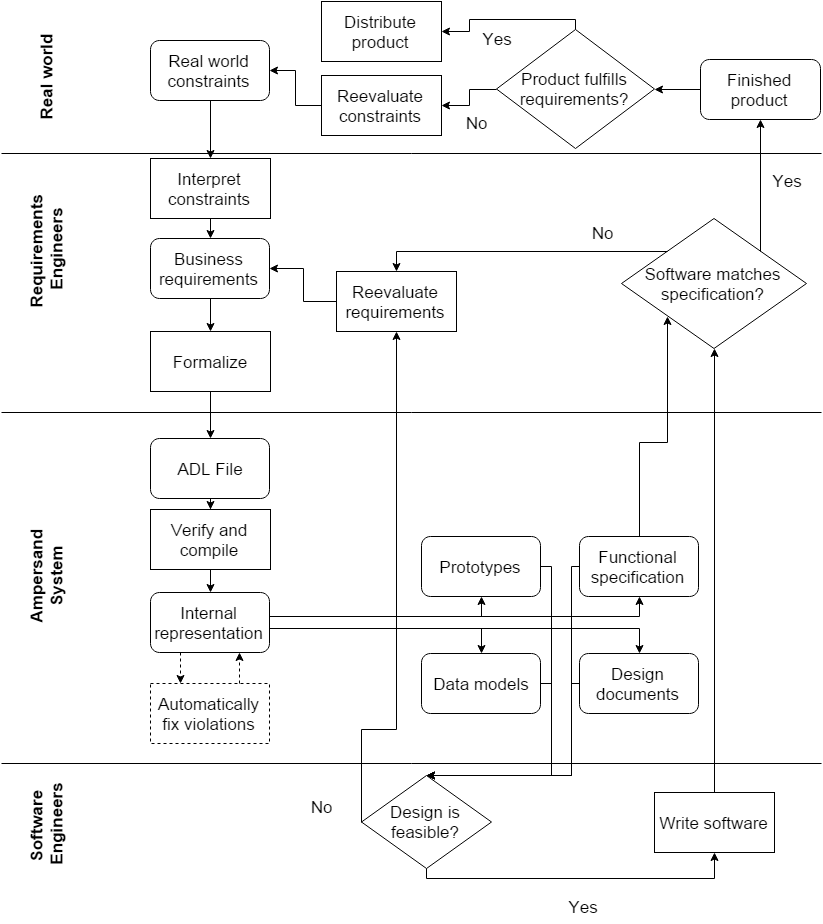
\includegraphics[width=\textwidth]{../figures/business_process}
        \caption{Business process diagram representing the role of Ampersand in 
        the software design cycle}~\label{fig:BusinessProcess} \end{center}
The diagram is a simplified view of the software design cycle, intended to 
highlight 
the role of Ampersand in this cycle. This view omits many of the uses of the 
design artifacts generated by Ampersand; instead it focuses mainly on the 
primary purpose, which is to help create a finished software system. 

The contribution of this project is denoted with dashed lines. Note that it is
isolated to a process completely internal to Ampersand.    
\end{figure}


\section{The Scope of the Work}\label{sec:ScopeOfWork}
The following sections focuses specifically on EFA and how it will 
function in the Ampersand environment.
%data flow diagram for EFA goes here
EFA is an automated process internal to Ampersand, and as a part of the 
Ampersand system it works in collaboration with other internal components such 
as the F-spec. The purpose of EFA is to replace the current exec-engine,
\edcomm{YT}{No explanation of ``exec-engine'' yet. It must be explained. Also, for the 
  sake of consistency, it should be written ``ExecEngine''. 
}
creating a permanent solution for the implementation of ECA rules. EFA also 
provides extensive functionalities that the exec-engine is missing, such as the 
ability to manipulate data in a database beyond the basic level of creating and 
dropping tables, and basic select queries. It provides the fundamental 
datatypes that are crucial for the expansion and maintenance of Ampersand as it 
grows. Due to the way that queries are generated in its present state, large 
number of projects will bog down the system until it becomes unmanageable, and 
if Ampersand is used in practice.

\subsection{The Current Situation} %what is being replaced/made better, the 
%effects of the proposed change

Ampersand currently has an exec-engine 

\edcomm{YT}{``an'' ExecEngine? ExecEngine is a proper noun. What is ``the'' ExecEngine?
}
that passes SQL queries which are 
triggered by the prototype user interface implemented in PHP. Though the 
exec-engine functions, it is a temporary solution for translating ECA rules 
into SQL queries. Any changes made to the information system after its initial 
generation require manual maintenance. This project will create a permanent 
solution that is provably correct and will automate the correction of system 
invariants so that manual maintenance of system invariants is no longer 
necessary once EFA has been successfully incorporated into Ampersand.

\section{The Scope of the Product}\label{sec:ScopeOfProduct}

\eddelete{YT}{
The translation of ECA rules into SQL queries require unique data types that 
preserves the semantics the user provides in the ADL script. ECA rules are 
generated from the conditions the user specifies in the ADL script. The SQL 
queries generated from ECA rules can be thought of as a sequence of changes 
made to the data. This sequence of actions are made through specific event 
triggers, and the actions only take place if all conditions are satisfied and 
are valid. An example of this, would be attempting to delete a person who does 
not exist. This actions cannot be completed because the person does not exist, 
this action would be invalid. 
}

\edcomm{YT}{This says NOTHING about the scope of the product! See ``writing random shit''} 

\section{Functional Requirements}\label{sec:Functional}
\ds{What about error handling on the new contributions?
    Where's the functional requirement related to: 
    ``be a pure function; it should not have side effects." and 
    ``provide diagnostic information about the algorithm to
    the user, if the user asks for such information."?}

\subsection{System Requirements}
%%-----------------------------SIDE EFFECTS---------------------------------%%
{\setlength{\tabcolsep}{6pt} %% Default is 6
    \begin{tabularx}{\textwidth}{>{\bfseries}m{3cm}X}
        Requirement & S1 \\ 
        \midrule
        \endhead
        Description  & Create pure functions with no unintended side effects
        \\	Rationale & The use of a functional programing languages requires 
        that this program be a pure function and does not have side effects, 
        however certain portions of the code requires the execution of side 
        effects to match the behaviour presented by external programs. In these 
        specific instances, the side effects are an intended behaviour.
        \\	Originator & Stakeholder/Developer
        
        \\	Fit Criterion & This behaviour is necessary to produce the results 
        the stakeholders desire
        \\ Test Case & Desired results can be confirmed as they will be 
        reflected in changes that take place in the Ampersand database.
        \\	Customer Satisfaction & 5 - Highest 
        \\	Priority & 5 - Highest 
        \\	Supporting Materials & (Rule Based Design \cite {RBD})
        \vspace{12pt}
    \end{tabularx}
}

%%------------------USE OF HASKELL AS IMPLEMENTATION LANGAUGE-----------------%%
{\setlength{\tabcolsep}{6pt} %% Default is 6
    \begin{tabularx}{\textwidth}{>{\bfseries}m{3cm}X}
        Requirement & S2 \\ 
        \midrule
        \endhead
        Description  & The use of Haskell to implement EFA modules
        \\	Rationale & The source code of Ampersand is written completely in 
        Haskell, and thus Haskell must be used for any modules created by this 
        project to be absorbed into the pre-existing source code.
        \\	Originator & Ampersand Creators (i.e. our client)        
        \\	Fit Criterion & Primary ability to write code compatible with 
        Ampersand as it is.
        \\ Test case & Added modules are tested with cabal build inside of 
        Ampersand
        \\	Customer Satisfaction & 5 - Highest 
        \\	Priority & 5 - Highest 
        \\	Supporting Materials & Dr. Joosten, Joosten and Kahl
        \vspace{12pt}
    \end{tabularx}
}
%%------------------ MODULES MUST FIT AMPERSAND FRAMEWORK-----------------%%
{\setlength{\tabcolsep}{6pt} %% Default is 6
    \begin{tabularx}{\textwidth}{>{\bfseries}m{3cm}X}
        Requirement & S3 \\ 
        \midrule
        \endhead
        Description  & Added modules must fit within Ampersand's current 
        framework
        \\	Rationale & As Ampersand is a huge system that has weekly additions 
        to prevent conflict and breaking of existing packages/modules, an 
        effort should be made to minimize external dependencies. As EFA will be 
        an internal component of Ampersand, if a package that EFA depends on to 
        function properly is no longer maintained and breaks, it will in turn 
        break Ampersand.
        \\	Originator & Ampersand Creators (i.e. our client)        
        \\	Fit Criterion & Functionality of EFA as an Ampersand internal 
        component.
        \\ Test case & Added modules are tested with cabal build inside of the
        Ampersand system as an internal component (i.e. System testing)
        \\	Customer Satisfaction & 4 - High 
        \\	Priority & 4 - High
        \\	Supporting Materials & Hackage, Dr. Kahl
        \vspace{12pt}
    \end{tabularx}
}
%%----------------------- MACHINE--------------------------------------------%%
{\setlength{\tabcolsep}{6pt} %% Default is 6
    \begin{tabularx}{\textwidth}{>{\bfseries}m{3cm}X}
        Requirement & S4 \\ 
        \midrule
        \endhead
        Description  & Machine-checked proofs
        \\	Rationale & EVA data-types are indexed on Haskell types, and 
        indices are selected in a way that impossible values are eliminated by 
        Haskell's strong type system.
        \\	Originator & Stakeholder/Developer
        
        \\	Fit Criterion & Program compiles and provides an inductive proof 
        that the SQL generated by ECA2SQL is correct
        \\ Test Case & Verified by examination
        \\	Customer Satisfaction & 5 - Highest 
        \\	Priority & 5 - Highest 
        \\	Supporting Materials & Requirement solicitation.
        \vspace{12pt}
    \end{tabularx}
}
\subsection{Project Requirements}
%%-------------------------TYPE CORRECTNESS ----------------------------------%%
{\setlength{\tabcolsep}{6pt} %% Default is 6
    \begin{tabularx}{\textwidth}{>{\bfseries}C{3cm}X}
        Requirement & P1 \\ 
        \midrule
        \endhead
        Description  & Provable Correctness: Haskell like other functional 
        programming languages have 
        a strong type system which can be used for machine-checked proofs.
        \\	Rationale & Curry-Howard correspondence which states that the 
        return type of the function is analogous to a logical theorem, that is 
        subject to the hypothesis corresponding to the types of the argument 
        values that are passed to the function and thus the program uysed to 
        compute that function is analogous to a proof of that theorem.
        \\	Fit Criterion & Provable correctness of the program that is 
        generated.
        \\ Test Cases & Internal structure of ECA rules can be compared to SQL 
        queries through a series of datatype tests, each of which will result 
        in a traceable result or error message
        \\	Priority & 4 - High
        \\	Supporting Materials & Programming language theory, Dr. Kahl
        \vspace{12pt}
    \end{tabularx}
}
%%--------------------------CORRECTNESS OF ECA TO SQL RULES ------------------%%
{\setlength{\tabcolsep}{6pt} %% Default is 6
    \begin{tabularx}{\textwidth}{>{\bfseries}C{3cm}X}
        Requirement & P2 \\ 
        \midrule
        \endhead
        Description  & Generated SQL queries must preserve the semantics of ECA 
        rules.  
        \\	Rationale & The translation would otherwise not be correct, as the 
        rules would be meaningless if their semantics are lost.
        \\	Originator & Ampersand Developers
        \\	Fit Criterion & Generated queries must be provably correct as per 
        client's request.
        \\ Test Cases & Internal structure of ECA rules can be compared to SQL 
        queries through a series of datatype tests, each of which will result 
        in a traceable result or error message
        \\	Priority & 4 - High
        \\	Supporting Materials & Hackage, Dr. Kahl
        \vspace{12pt}
    \end{tabularx}
}
%%-------------------------TRACABLE EERRORS---------------------------%%
{\setlength{\tabcolsep}{6pt} %% Default is 6
    \begin{tabularx}{\textwidth}{>{\bfseries}C{3cm}X}
        Requirement & P3 \\ 
        \midrule
        \endhead
        Description  & Generating traceable results and error messages for 
        handling new contributions from this project
        \\	Rationale & Saves time by allowing the program to inform the 
        programmer where the errors are located.
        \\	Originator & Ampersand Developers
        \\	Fit Criterion & Errors must be traceable and have a standard format 
        that can be easily followed.
        \\ Test Cases & Error message will print to screen.
        \\	Priority & 4 - High
        \\	Supporting Materials & Hackage, Dr. Kahl
        \vspace{12pt}
    \end{tabularx}
}

\subsection{Non-Functional Requirements}
%%---------------------------AVAILABILITY TO USERS REQUIREMENT ---------------%%
{\setlength{\tabcolsep}{6pt} %% Default is 6
\begin{tabularx}{\textwidth}{>{\bfseries}C{3cm}X}
Requirement & N1 \\ 
\midrule
\endhead
Description  & EFA must be available at anytime Ampersand is running.
\\	Rationale & To provide the user with unlimited access to EFA within 
Ampersand.
\\	Originator & Ampersand Developers
\\	Fit Criterion & Ampersand can detect when internal components are 
non-responsive
\\ Test cases & Ampersand is subject to sentential tests on a daily basis as 
part of its maintenance.   
\\	Priority & 4 - High
\\	Supporting Materials & Useful feedback in Ampersand parser \cite{SB2011}
\vspace{12pt}
\end{tabularx}
}


\chapter{Non-Functional Requirements}\label{ch:NonFunc}
\begin{figure}[!htb]
	\centering
	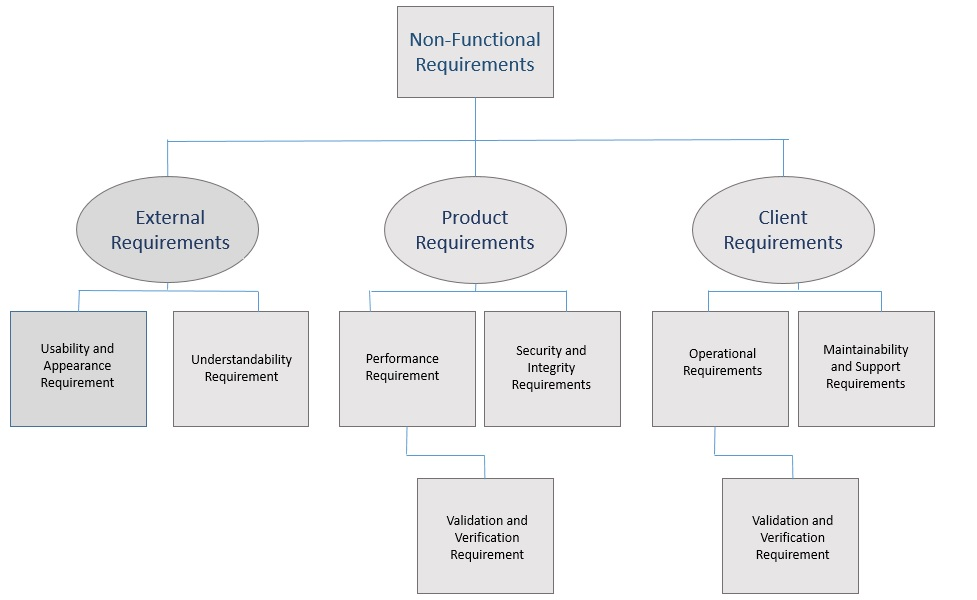
\includegraphics[width=0.8\textwidth]{../figures/NONFUNCTIONAL}
	\caption{Tree of non-functional requirements as it relates to 
	EFA}~\label{fig:figure2} 
\end{figure}
    Each Non-functional requirement must be traceable in the Ampersand system 
    with the addition of EFA. 
\edcomm{YT}{If we make this claim we better provide data and facts to 
  back up the traceability. Have we done this? No. Will we be able to do it? 
  Probably not easily}
    \textit{Note: Missing sections in this chapter are not applicable for this 
    project }    
\edcomm{YT}{Not necessary. A document about any topic is assumed to not include 
  information not relevant to that topic. On the subject of missing sections, 
  please put them all back in. The flow and organization of this document 
  has degraded to essentially zero with all of the removals and renmaings 
  and mysterious changes.}

\section{Performance Requirements}\label{sec:Performance}
\paragraph*{}
EFA is designed to optimize 
\edcomm{YT}{``optimize'' is not the right word here}
the Ampersand system by automating the tedious task 
of restoring system invariants when broken using ECA rules. 
Ampersand will 
perform as it use to with less maintenance required on behalf of the user.
\edcomm{YT}{Is this even a sentance?}


\section{Maintainability and Support Requirements}\label{sec:Support}
\paragraph*{}
EFA must make sure that each specification/error is traceable 
(\cite[2]{derFun}). EFA will be upgrade and tested as a part of Ampersand does 
not require additional maintenance or support to perform optimally.

\edcomm{YT}{Both the grammar and content of this section is bad} 

\section{Validation and Verification Requirements}\label{sec:Verification}



\edcomm{YT}{This table is very poorly formatted. If you use tables,
  they must look good. Firstly your things need to fit into the table 
  properly. Secondly, please do not place so many rules everywhere 
  and do not put a box around the table for no reason. You should 
  strive to MINIMIZE your use of rules, not maximize. Please fix 
  ALL of the hideous tables. Thirdly, DO put a title and caption 
  on EVERY SINGLE TABLE. To be clear, THIS IS ABSOLUTELY NECESSARY.
  In general, tables are a terrible organization structure 
  for English prose, so this table should just be removed and the information 
  organized into a logical format, like paragraphs. Next onto the 
  content. Every explanation that is a few words is correct. Every single
  one which is longer is either simply WRONG or is just completely
  nonsensical. Secondly, most, if all, of these things do NOT need
  to be introduced. Thirdly, the organization of the information 
  is just poor - there is a definition for ``X : Y where Y $\in$ Type,Kind''
  however the given definition only holds in the context of a declaration
  and only when explicitly giving things which are definitional equal 
  to themselves. The entry as written implies that the syntax ``X : Y'' 
  has this meaning, which is clearly untrue. `where Y $\in$...' is not part of 
  the syntax, so it shouldn't be written so simply beside the part 
  which IS real syntax, because it misleads the reader into thinking 
  that the entire thing is real syntax. If you do write this, there 
  should be a logical seperator between the two, for example writing 
  one of them in a different font. Fourthly, if this information 
  is placed anywhere, it certainly should NOT be in the functional requirements 
  section. It should be in the same section, or adject to, as the part
  where we describe terminology. } 

\begin{longtable}{|m{5cm}|m{9cm}| }
    \hline 
    \textbf{Notation}  & \textbf{Description} \\ \hline
       X : Y   &  X has type Y \\ 
        \hline  
       $`Types`$  &  Type of types \\ 
        \hline
       $`Kind`$   &  Type of Kinds \\ 
        \hline
         \_ $\rightarrow$ \_ ∶ Type →$\rightarrow$Type $\rightarrow$ Type  & 
         This function requires 2 Type inputs and produces a Type output. Where 
         \_ $\rightarrow$ \_ can be seen as for each element x of type A 
         defines a function F(x) where x does not exist in set {Type,Kind} for 
         every x that defines F(x)  \\ 
        \hline
       \_ $\rightarrow$ \_∶ Kind $\rightarrow$Kind $\rightarrow$ Kind  & This 
       function requires 2 of type Kinds and produces an output of Type Kinds . 
       Where 
       \_ $\rightarrow$ \_ can be seen as for each element x of type A 
       defines a function F(x) where x does not exist in set {Type,Kind} for 
       every x that defines F(x). This a dependent type, an example of this 
       would be 
       SingT (x :: a) $\rightarrow$ SingT (F x)
       \\ 
        \hline
          $\mathbb{N}$, Symbol : Kind   &  Left of the : are the elements that 
          represent type Kinds (right of the : )\\ 
        \hline
          0, 1, 2, $...$ ∶ $\mathbb{N}$   &  These are natural numbers, 
          elements left of the : belong to the set N of natural numbers\\ 
        \hline
         \{$""$, $"a"$, $"aa"$, $...$, $"b"$, $"bb"$\} : Symbol &  
         Elements left of : are elements that belong to the set Symbol \\ 
        \hline
        ( x : A  ) $\rightarrow$ F x   & \\ where x $\notin$ \{Type,Kind\}   &  
        This can also be seen as $\forall$ x $\rightarrow$ F x; where as  \\ 
        \hline
           SingT \(x $::$ a\) $\rightarrow$ SingT \(F x\)  &  SingT is the type 
           of singleton, a dependent type created for EFA datatypes. \\ 
        \hline
          $\rightarrow$: Constraint $\rightarrow$ Type $\rightarrow$ Type  and  
          \_ $\Rightarrow$ \_ : Type $\rightarrow$ Constraint $\rightarrow$ 
          Type    &  where $\forall$x : S $\Rightarrow$ T corresponds to 
          $\mathbf{G}$ \textit{S} ($\lambda$x.T) in Illative Combinatory 
          Logic 
          where G is the combinator \cite{CombLogic}. The $\Rightarrow$ 
          represents restraints for what on the right side of the : .\\ 
        \hline
        X : Y  where Y $\in$ {Type,Kind} &  X is equal in definition to 'X : 'Y 
        and only X' : Y'. \\ 
        \hline
        elim-Y: (r:Type) $\rightarrow$ Y $\rightarrow$ ($A_0$ $\rightarrow$ r) 
        $\rightarrow$ ($A_1$ $\rightarrow$ r ) $\rightarrow$ $\rightarrow$ 
        $...$ $\rightarrow$ ($A_n$ $\rightarrow$ r) $\rightarrow$ r   &  An 
        eliminator that corresponds to pattern matching \\ 
        \hline
        'P : Y $\rightarrow$ Z'   &  This represents 'P (Ctr x)', where 'Ctr  
        is used for type casting\\ 
        \hline
         $\exists$ (x : A) (P x) & This indicates that (r:Type) $\rightarrow$ 
         ((x:A) . (P x $\rightarrow$ r) $\rightarrow$ r) \\ 
        \hline
        X : Y   &  X has type Y \\ 
        \hline
        
\end{longtable}

\section{Module Decomposition}
\textit{Note: * represents the top level module}
\begin{figure}[!htb]
    \centering
    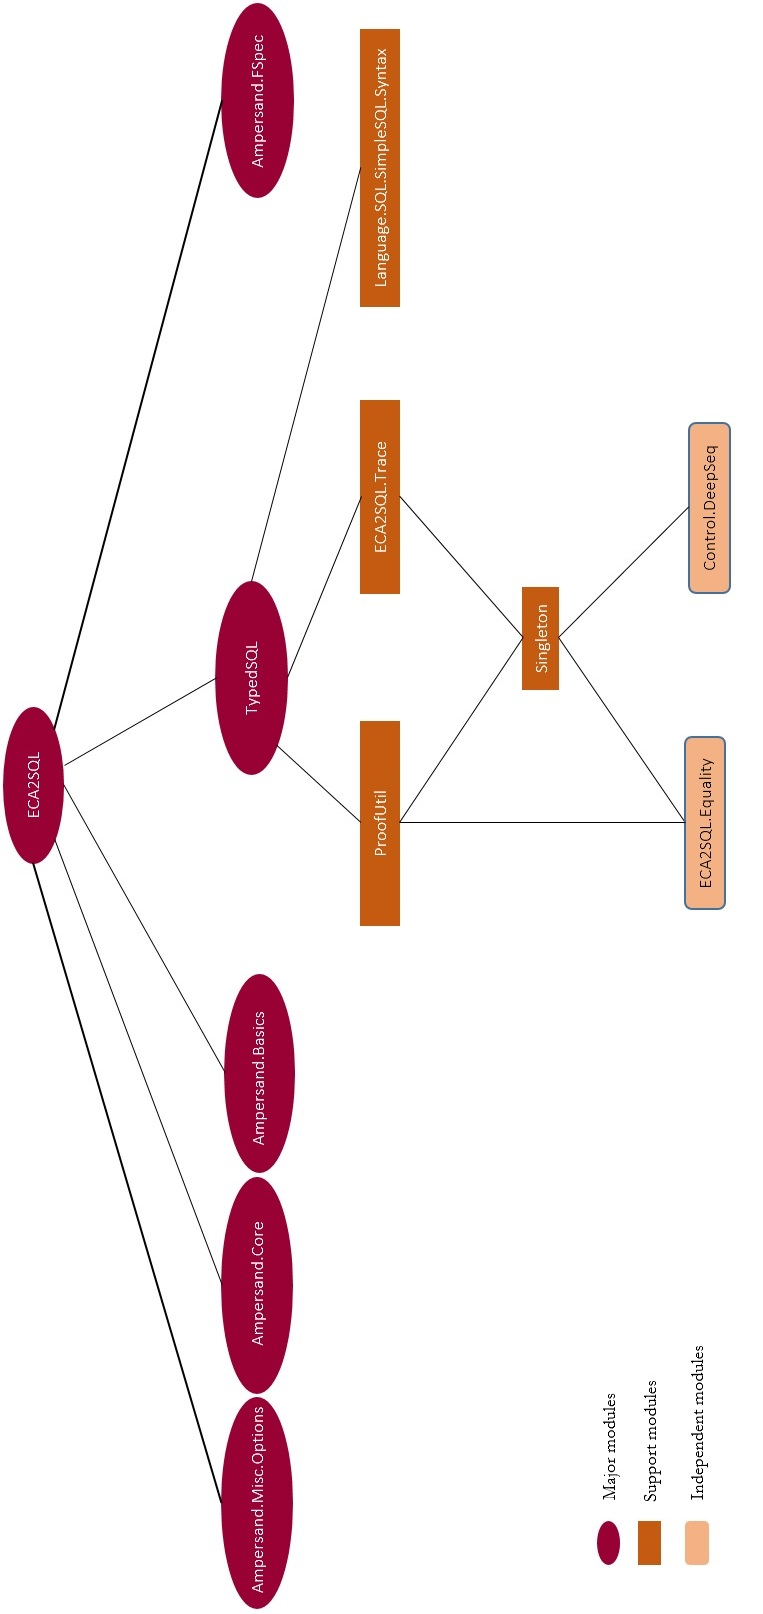
\includegraphics[width=0.65\textwidth]{../figures/projTree}
    \caption{Hierarchy of EFA Modules
        EFA}~\label{fig:figure2} 
\end{figure}

\edcomm{YT}{Full page figures go in the appendix at the end, Preferably fit it into 
  the page width}

\newpage

\edcomm{YT}{I understand this is unfinished but the same comments about table formatting apply.
  Also this table goes *far* outside of the margins of the page. This is very bad. 
  Finally, this data is not a good fit for a table either (diagrams are your friend)}

\setlength\LTleft{-1in}
\setlength\LTright{-1in}
\begin{longtable}{|m{1.5cm}|m{2.5cm}|m{6cm}|m{6cm}|} \hline
 \textbf{Module}  & \textbf{Functions} &\textbf{Function Types} & 
 \textbf{Description} \\ \hline \hline
    ECA2SQL  & eca2SQL  & Options $\rightarrow$ FSpec $\rightarrow$ ECArule 
    $\rightarrow$ SQLMethod '[] 'SQLBool & d \\ 
    \hline
    ECA2SQL  & eca2PrettySQL  &  Options $\rightarrow$ FSpec $\rightarrow$ 
    ECArule $\rightarrow$ Doc  & d \\ 
    \hline \hline
    a  & b  & c & d \\ 
    \hline
    a  & b  & c & d \\ 
    \hline
    a  & b  & c & d \\ 
    \hline
    a  & b  & c & d \\ 
    \hline
    a  & b  & c & d \\ 
    \hline
    a  & b  & c & d \\ 
    \hline
    a  & b  & c & d \\ 
    \hline
    a  & b  & c & d \\ 
    \hline
    a  & b  & c & d \\ 
    \hline
\end{longtable}
%%%%%%%%%%%%%%%%%%%%%%%%%%%%%%%%%%%%%%%%%%%%%%%%%%%%%
\chapter{Project Issues}\label{ch:issues}
\vspace{-1cm}
\textit{Sections not applicable to this project have been removed}

\edcomm{YT}{Put them back}

\section{Tasks}\label{sec:Tasks}
\begin{itemize}
\item Translate ECA rules to SQL commands
\item Create supporting data structures for sustainable translation and future 
maintenance
\item Implement the solution and provide the  annotated source code to the supervisor and the product owner for a review.
\item Incorporate changes to project as suggested by our client and supervisor
\item Provide provable correctness for program
\end{itemize}
\edcomm{YS}{Add in any significant task you feel is worth mentioning}%
\section{Migration to the New Product}\label{sec:Migration}
\paragraph*{}
Upon final review by the client and intensive testing, if the client is
satisfied by the quality of code and its maintainability, the implementation
will be made part of the production stream hosted on Github.  
\section{Risks}\label{sec:Risks}
\begin{itemize}
\item The new code must not introduce any errors or performance regressions
into Ampersand.
\item The code must satisfy existing tests and additional tests written for the 
new algorithm being implemented.
%%I'm pretty sure more goes here
\end{itemize}

\section{Costs}\label{sec:Costs}
\paragraph*{}
The cost is eight months of time.

\section{User Documentation and Training}\label{sec:UserDoc}
\paragraph*{}
User documentation is not necessary, as EFA provides traceable error messages 
for developers. 


\bibliographystyle{alpha}
\bibliography{SRS}
\end{document}










